%نام و نام خانوادگی:
%شماره دانشجویی: 
\مسئله{مقایسه‌ی \lr{LR(1)} و \lr{SLR(1)}}

\پاسخ{ }
\\\\
الف) قسمتی از متن غلط است. در SLR(1) از Follow غیرپایانه ها استفاده میشود و در LR(1) از LookAhead‌ اما دقت SLR کمتر است، زیرا در SLR فقط به Follow غیرپایانه ها توجه داریم ولی در LR(1) به فراتر از آن توجه می‌کنیم یعنی LA (Lookahead) ها. LA ها ممکن است در دو جای مختلف برای دو قاعده تولید یکسان، متفاوت باشند. برعکس Follow ها که برای دو قاعده یکسان، لزوما یکسان اند. بنابراین LR(1) دقت بیشتری در تمییز دادن حالت های مختلف، نسبت به SLR(1) دارد. همچنین LR(1) فضای بیشتری اشغال میکند، چون تعداد زیادی state داریم که یک قاعده تولید یکسان ممکن است در هرکدام با LA های مختلف ظاهر شود. اما در SLR به اندازه LR(0) فضا اشغال میشود و یک قاعده تولید نمی تواند به اشکال مختلف در state های مختلف ظاهر شود، زیرا Follow غیرپایانه سمت چپ آن به هر حال ثابت است و در نتیجه می‌توان صرفا یک جدول داشت که Follow هر non-terminal در آن ذخیره شده است و با رجوع به آن Follow مورد نظر را بفهمیم.
\\\\
ب) عکس دیاگرام SLR(1)در زیر نمایش داده شده است:
\graphicspath{{./images/}}
\begin{center}
	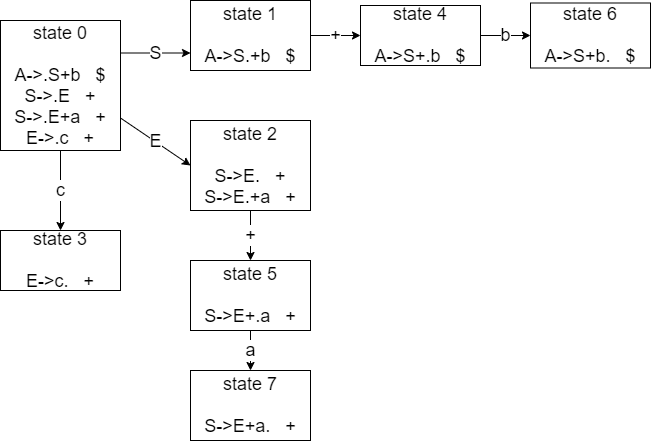
\includegraphics[scale=0.7]{compiler_hw2_q10_1}
\end{center}
عکس دیاگرام LR(1) در زیر نمایش داده شده است:
\graphicspath{{./images/}}
\begin{center}
	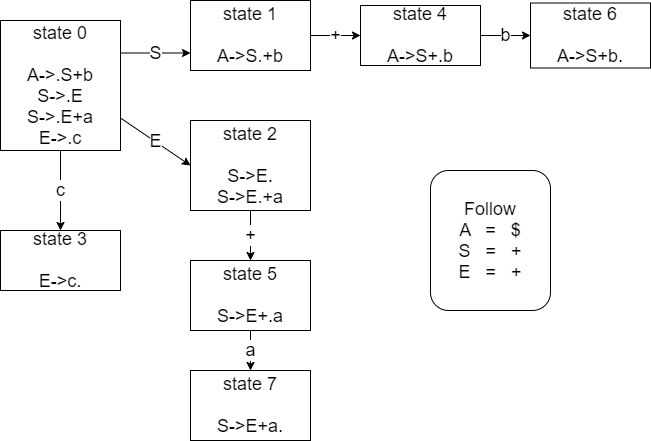
\includegraphics[scale=0.7]{compiler_hw2_q10_2}
\end{center}
گرامر نه SLR(1) هست و نه LR(1)‌ .
\\
SLR(1)
به این دلیل نیست که در استیت شماره ۲، با ترمینال + هم می‌توان به استیت شماره ۵ shift کرد و هم می‌توان با قاعده تولید شماره ۲ reduce کرد چون + در follow غیرپایانه S وجود دارد.
\\
LR(1) 
هم به دلیل مشابه نیست. در استیت شماره ۲، با ترمینال + هم می‌توان به استیت شماره ۵ shift کرد و هم می‌توان‌ با قاعده تولید شماره ۲ reduce کرد و + در lookahead های این قاعده وجود دارد.
